\documentclass[serif]{beamer}\usepackage[]{graphicx}\usepackage[]{color}
%% maxwidth is the original width if it is less than linewidth
%% otherwise use linewidth (to make sure the graphics do not exceed the margin)
\makeatletter
\def\maxwidth{ %
  \ifdim\Gin@nat@width>\linewidth
    \linewidth
  \else
    \Gin@nat@width
  \fi
}
\makeatother

\definecolor{fgcolor}{rgb}{0.345, 0.345, 0.345}
\newcommand{\hlnum}[1]{\textcolor[rgb]{0.686,0.059,0.569}{#1}}%
\newcommand{\hlstr}[1]{\textcolor[rgb]{0.192,0.494,0.8}{#1}}%
\newcommand{\hlcom}[1]{\textcolor[rgb]{0.678,0.584,0.686}{\textit{#1}}}%
\newcommand{\hlopt}[1]{\textcolor[rgb]{0,0,0}{#1}}%
\newcommand{\hlstd}[1]{\textcolor[rgb]{0.345,0.345,0.345}{#1}}%
\newcommand{\hlkwa}[1]{\textcolor[rgb]{0.161,0.373,0.58}{\textbf{#1}}}%
\newcommand{\hlkwb}[1]{\textcolor[rgb]{0.69,0.353,0.396}{#1}}%
\newcommand{\hlkwc}[1]{\textcolor[rgb]{0.333,0.667,0.333}{#1}}%
\newcommand{\hlkwd}[1]{\textcolor[rgb]{0.737,0.353,0.396}{\textbf{#1}}}%
\let\hlipl\hlkwb

\usepackage{framed}
\makeatletter
\newenvironment{kframe}{%
 \def\at@end@of@kframe{}%
 \ifinner\ifhmode%
  \def\at@end@of@kframe{\end{minipage}}%
  \begin{minipage}{\columnwidth}%
 \fi\fi%
 \def\FrameCommand##1{\hskip\@totalleftmargin \hskip-\fboxsep
 \colorbox{shadecolor}{##1}\hskip-\fboxsep
     % There is no \\@totalrightmargin, so:
     \hskip-\linewidth \hskip-\@totalleftmargin \hskip\columnwidth}%
 \MakeFramed {\advance\hsize-\width
   \@totalleftmargin\z@ \linewidth\hsize
   \@setminipage}}%
 {\par\unskip\endMakeFramed%
 \at@end@of@kframe}
\makeatother

\definecolor{shadecolor}{rgb}{.97, .97, .97}
\definecolor{messagecolor}{rgb}{0, 0, 0}
\definecolor{warningcolor}{rgb}{1, 0, 1}
\definecolor{errorcolor}{rgb}{1, 0, 0}
\newenvironment{knitrout}{}{} % an empty environment to be redefined in TeX

\usepackage{alltt}
\usetheme{EPA}
\usepackage{graphicx}
\usepackage{xcolor}
\usepackage{tikz}
\usetikzlibrary{decorations.pathreplacing}
\usetikzlibrary{shapes,arrows,positioning,trees,shadows}


%tikz objects
\tikzstyle{decision} = [diamond, draw, text width=6em, text badly centered, node distance=3cm, inner sep=2pt, top color=white, bottom color=green!25]
\tikzstyle{block} = [rectangle, draw, text width=10em, text centered, rounded corners, minimum height=3em, minimum width=8em, top color = white, bottom color=blue!30,  drop shadow]
\tikzstyle{declare} = [rectangle, draw, text width=10em, text centered, minimum height=3em, minimum width=8em, top color = white, bottom color=orange!30,  drop shadow]

% macros
\newcommand{\emtxt}[1]{\textbf{\textit{#1}}}

% knitr setup


\IfFileExists{upquote.sty}{\usepackage{upquote}}{}
\begin{document}

%%%%%%
\begin{frame}{Path to EPA}
\setbeamercovered{again covered={\opaqueness<1->{45}}}
\onslide<1->{
{\bf Dr. Marcus W Beck}, Ecosystem Ecologist and Data Scientist \\~\\
}
\begin{columns}[t]
\begin{column}{0.35\textwidth}
\onslide<2>
\underline{\textbf{2002-2009}}\\~\\
\begin{itemize}
\item BSc in Zoology \\~\\
\item Intern for Florida FWC \\~\\
\item MSc in Conservation Biology \\~\\
\end{itemize}
\end{column}
\begin{column}{0.35\textwidth}
\onslide<3>
\underline{\textbf{2010-present}}\\~\\
\begin{itemize}
\item Intern for Minesota DNR \\~\\
\item PhD in Conservation Biology \\~\\
\item Post-doc at GED \\~\\
\end{itemize}
\end{column}
\end{columns}
\end{frame}

%%%%%%
\begin{frame}[t]{My interests}

% \setbeamercovered{again covered={\opaqueness<1->{45}}}
\begin{columns}[T]
\begin{column}{0.5\textwidth}
  \begin{itemize}
  \setlength\itemsep{1.5em}
    \only<1>{ 
      \item Water quality
      \item Biological monitoring
      \item Eutrophication
      \item Aquatic Macrophytes
      \item Ecosystem metabolism
    }
    \only<2>{
      \item Indicator development
      \item Time series methods
      \item Reproducible research
      \item Visualization and graphics
      \item Model comparisons
    }
    \only<3->{
      \item NeuralNetTools
      \item SWMPr
      \item WtRegDO
      \item WRTDStidal
      \item ggord
      \item rStrava
    }
  \end{itemize}
\end{column}

\begin{column}{0.4\textwidth}
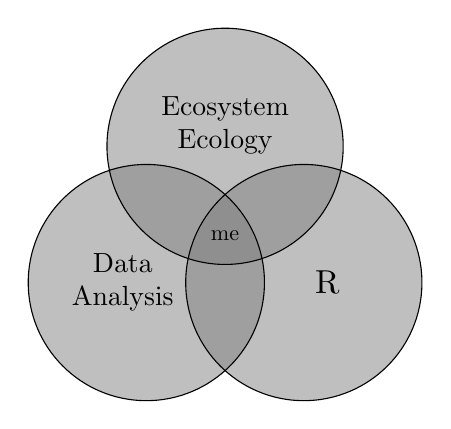
\begin{tikzpicture}
  \begin{scope}

    % The transparency:
    \begin{scope}[fill opacity=0.5]
      \onslide<2->\fill[gray] (-1, 0) circle (1.5);
      \onslide<3->\fill[gray] (1, 0) circle (1.5);
      \onslide<1->\fill[gray] (0, 1.73) circle (1.5);
    \end{scope}
    
    % letterings and missing pieces:
    \onslide<2->\draw[align=center] (-1, 0) circle (1.5);
    \onslide<3->\draw[align=center] (1, 0) circle (1.5);
    \onslide<1->\draw[align=center] (0, 1.73) circle (1.5);
    \onslide<2->\draw (-1.3, 0) node[scale=1,align=center] {Data \\ Analysis};
    \onslide<3->\draw (1.3, 0) node[scale=1.2] {R};
    \onslide<1->\draw (0, 2) node[scale=1,align=center] {Ecosystem \\ Ecology};
 		\onslide<4->\draw (0, 0.6) node[scale=0.8] {me};
 		
  \end{scope}
\end{tikzpicture}
\end{column}
\end{columns}
\end{frame}

%%%%%%
\begin{frame}[t]{Past work - Biological assessment of lakes}
\onslide<+->{How appropriate is a biological index for characterizing effects of multiple stressors? Will it work within a regulatory framework?\\~\\}
\onslide<+->{
\vspace*{-0.1in}
\begin{center}
\scalebox{0.6}{
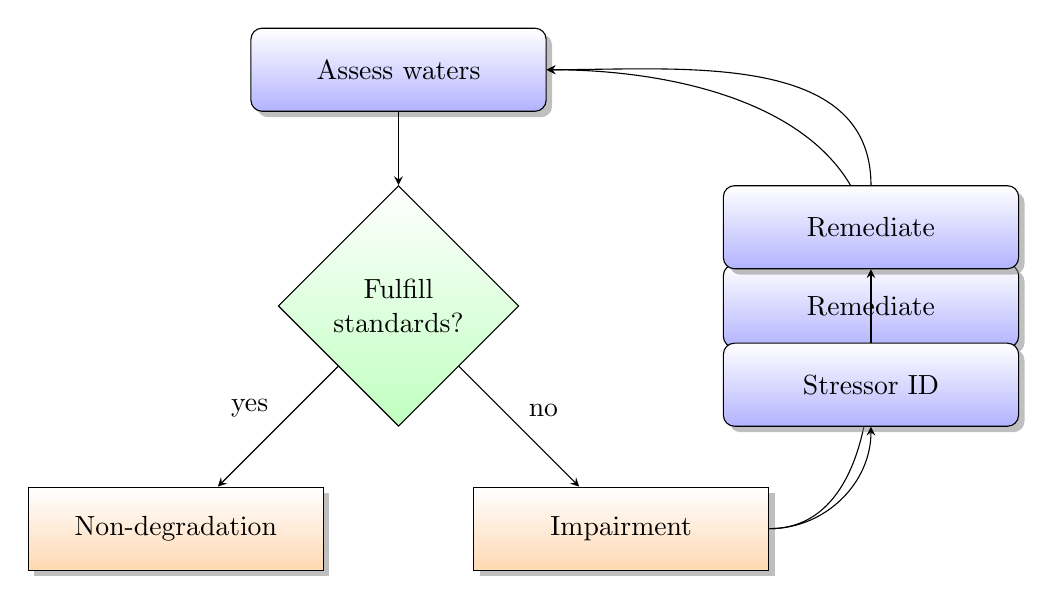
\begin{tikzpicture}[node distance=2.5cm, auto, >=stealth]
	\node[block] (a) {Assess waters};
	\onslide<+->{
	\node[decision] (b)  [below of=a] {Fulfill standards?};
 	\draw[->] (a) -- (b);}
 	\onslide<+->{
 	\node[declare] (c)  [below left of=b, node distance=4cm]  {Non-degradation};
 	\draw[->] (b) -- node[above left] {yes} (c);}
 	\onslide<+->{
 	\node[declare] (d)  [below right of=b, node distance=4cm]  {Impairment};
 	\draw[->] (b) -- node[above right] {no} (d);}
 	\onslide<+>{
 	\node[block] (e)  [right of=b, node distance=6cm]    {Remediate};
 	\draw[->] (d.east) to [out=360,in=270] (e.south);
 	\draw[->] (e.north) to [out=90,in=360] (a.east);}
 	\onslide<+->{
 	\node[block] (f)  [below of=e, node distance=1cm]    {Stressor ID};
 	\node[block] (g)  [above of=e, node distance=1cm]    {Remediate};
	\draw[->] (d.east) to [out=360,in=270] (f.south);
	\draw[->] (f.north) to [out=90,in=270] (g.south);
 	\draw[->] (g.north) to [out=90,in=360] (a.east);}
\end{tikzpicture}}
\end{center}}
\end{frame}

% custom colors
\definecolor{mypal1}{HTML}{F0F9E8}\definecolor{mypal2}{HTML}{BAE4BC}\definecolor{mypal3}{HTML}{7BCCC4}\definecolor{mypal4}{HTML}{43A2CA}\definecolor{mypal5}{HTML}{0868AC}

\tikzstyle{decision} = [diamond, draw, text width=6em, text badly centered, inner sep = 2pt, top color=white, bottom color=mypal3, drop shadow]
\tikzstyle{block} = [rectangle, draw, text width=10em, text centered, rounded corners, minimum height=3em, minimum width=8em, top color = white, bottom color=mypal4,  drop shadow]
\tikzstyle{declare} = [rectangle, draw, text width=10em, text centered, minimum height=3em, minimum width=8em, top color = white, bottom color=mypal5,  drop shadow]

%%%%%%
\begin{frame}[t]{Current work - Evaluating estuarine condition}
How can we leverage monitoring data to develop our conceptual model of eutrophication? \\~\\
\onslide<+->
\begin{quote}
Eutrophication (noun) - an \emtxt{increase} in the rate of supply of \emtxt{organic matter} to an ecosystem\\
\end{quote}
\begin{center}
\scalebox{0.8}{
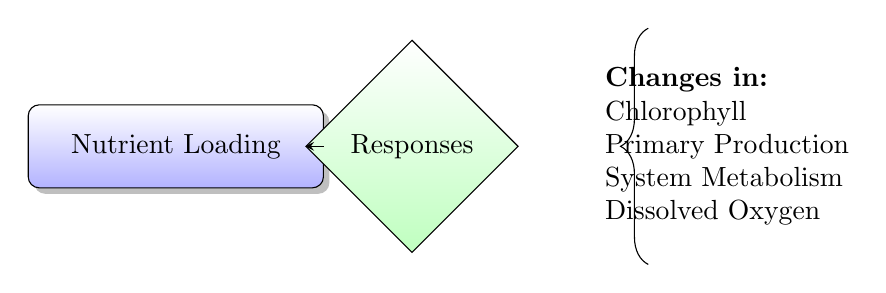
\begin{tikzpicture}[node distance = 4cm, auto, >=stealth]
  \onslide<+->{
  \node[block] (a) {Nutrient Loading};}
  \onslide<+->{
	\node[decision] (b)  [right of=a] {Responses};
 	\draw[->] (a) -- (b);}
  \onslide<+->{
  \draw[decorate,decoration={brace,amplitude=10pt}] [right of=b] (2,-1.5) -- (2,1.5);
  \node[draw,align=left,draw=none] [right of=b] {\textbf{Changes in:}\\ Chlorophyll\\ Primary Production\\ System Metabolism\\ Dissolved Oxygen};}
\end{tikzpicture}}
\end{center}
\end{frame}

\end{document}
